\documentclass[a4paper]{article}

%% Font selection
\usepackage{DejaVuSerifCondensed, DejaVuSansCondensed, DejaVuSansMono}
\usepackage{microtype}
\usepackage[T1]{fontenc}

%% Listings (see https://www.ctan.org/pkg/minted for installation)
\usepackage[outputdir=.texpadtmp]{minted}
\setminted{	python3 = true,
			fontsize = \small, 
			frame = leftline, 
			framesep = 2\fboxsep}
\usepackage{upquote}  % TT quotes in listings

%% Other packages
\usepackage[english]{babel}  % Language support
\usepackage{graphicx, epstopdf}  % Support EPS figures
\epstopdfsetup{outdir=.texpadtmp/}
\usepackage{url, hyperref}  % \url command, properly working
\usepackage[style=ieee, isbn=false]{biblatex}  % Bibliography
\addbibresource{bibliography.bib}
\usepackage{framed}  % Enables frames around quote env.
 
%% Shortcuts
\usepackage{xspace}
\newcommand{\matlab}{\textsc{Matlab}\xspace}
\newcommand{\csv}{\texttt{CSV}\xspace}
\newcommand{\newpaper}[1]{\subsection{\cite{#1}. \citetitle{#1}}

\begin{framed}\begin{quote}\begin{description}
	\item [Author]\citeauthor{#1}
	\item [Title]\citetitle{#1}
	\item [Year]\citedate{#1}
\end{description}\end{quote}\end{framed}}

%% Last package of all
\usepackage{cleveref}  % Allows en­hanced cross-ref­er­enc­ing fea­tures

%% Document details
\title{Piecewise segmentation for financial data}
\author{Paolo Antonini \and Davide Azzalini \and Fabio Azzalini}
\date{}


\usepackage{lipsum}  %TODO REV Remove


%% DOCUMENT
\begin{document}

\maketitle
%TODO Riscrivi
\begin{abstract}
Time series data is characterised as large in data size, high dimensionality and update continuously. Moreover, the time series data is always considered as a whole instead of individual numerical fields. As a consequence, in order to analyse and mine time series data, segmentation and dimensionality reduction are essential. In particular, in the following pages we are going to collect and study some segmentation methods, applied in particular to stock market data. Stock time series has its own characteristics over other time series. 
\end{abstract}

\section{Introduction}
The tasks of segmentation and dimensionality reduction, as well as identification of trends, are fundamental to allow a number of time series analysis and mining tasks. As a matter of fact, the fields of application of such procedures are numerous (ECG, exchange rates, sensor detections of any kind, \dots) and methods differ from application to application, due to the characteristics of data. As a consequence, literature regarding these issues is vast. 

In particular, our focus is on stock market data, which is inherently large in size, noisy and continuously updated. In this paper we are going first to list some of the main research papers where dimensionality reduction and piecewise segmentation are studied, in \cref{sec:methods}. Then, in \cref{sec:implementations} we are going to present some implementations of the methods. 


\section{Methods}\label{sec:methods}
 
\lipsum[1-3]

\newpaper{Yu2006} \lipsum[2-4]


\section{Implementations}\label{sec:implementations}

\paragraph{Turning points} Due to its simplicity, the apparently good results and openness to further improvements, we decided to implement the \emph{turning points} method presented in \cite{5961935}. So, in the following \cref{sec:tp_matlab,sec:tp_python} we are presenting our implementation both in \matlab and in Python of the method.

Basically, the algorithm is divided into two phases. First, during a preprocessing phase all points which are neither local maxima nor minima are discarded; then some patterns are simplified, since immaterial. However, we are not going to discuss the theoretical foundations and the steps of the algorithm in detail, as the aforementioned article if sufficient.

\paragraph{Other implementations} In order to provide a better view on the implementations, we are presenting other methods in \cref{sec:other}. Most notably, ... %TODO Completare!



\subsection{Turning points in \matlab}\label{sec:tp_matlab}

\paragraph{Implementation} The method is developed and tested over \csv files downloaded from Yahoo! Finance website\footnote{\url{http://finance.yahoo.com/market-overview/}}. Should another source be used, basic adaptations may be necessary, mostly in the handling of temporal data\footnote{Due to our limited knowledge of Matlab language, we may have dealt with the source data in a na{\"i}ve way. Nevertheless, the procedure seems to work well.} (i.e., dates), which is performed in \texttt{TP\_prepareData()} procedure. 

After importing the aforementioned \csv file (we suggest to use the graphical interface provided by \matlab itself), the user should issue the following command, in order to compute and plot the results: \mint{matlab}{y = TurningPoints(time, values, n);}

Here, \texttt{time} and \texttt{values} represent the time series as imported from the \csv; \texttt{n} instead lets the user specify the number of times the algorithm shall be performed (preprocessing is excluded from this count). The results are both displayed in a plot and stored in \texttt{y} variable.

\texttt{TurningPoints()} function is implemented as shown in \cref{lst:turningPoints}, with the support of some side functions.

\clearpage % TODO Clearpage

\begin{listing}%[H]
 
\inputminted[firstline = 1, lastline = 50]{matlab}{../code/TurningPoints.m}

\caption{\texttt{TurningPoints()} function.}\label{lst:turningPoints}

\end{listing}

\clearpage % TODO Clearpage

The main supporting function is \texttt{TP\_preprocess()}, which implements the preprocessing phase, and is presented in \cref{lst:preprocess}. The other supporting functions are of secondary importance, so we are not presenting them here. Basically we have: \begin{itemize}
	\item \texttt{TP\_prepareData()} takes in input raw Yahoo! Finance data and prepares them to the processing;
	\item \texttt{TP\_cleaning()} cleans data matrix after processing;
	\item \texttt{TP\_output()} shows information about the processing (i.e., the number of deleted elements).
\end{itemize} 

\begin{listing}%[H]
 
\inputminted[firstline = 53, lastline = 78]{matlab}{../code/TurningPoints.m}

\caption{\texttt{TP\_preprocess()} supporting function.}\label{lst:preprocess}

\end{listing}


\paragraph{Test} To conclude our discussion, we are presenting some tests we performed. Weekly stock market data from A2A (\texttt{A2A.MI}) over the whole 2015 were used as source. In particular, we plotted the weekly \texttt{Close} time series. In \cref{fig:a2a_w_2015} we show the original data in blue, the preprocessed data in orange and the data after one full run of the algorithm in yellow. 

Original data contains 53 samples; preprocessing reduces them to 27, and finally, after the actual processing, only 12 samples are left. 

\clearpage % TODO Clearpage

\begin{figure}%[H]
	
	\makebox[\textwidth][c]{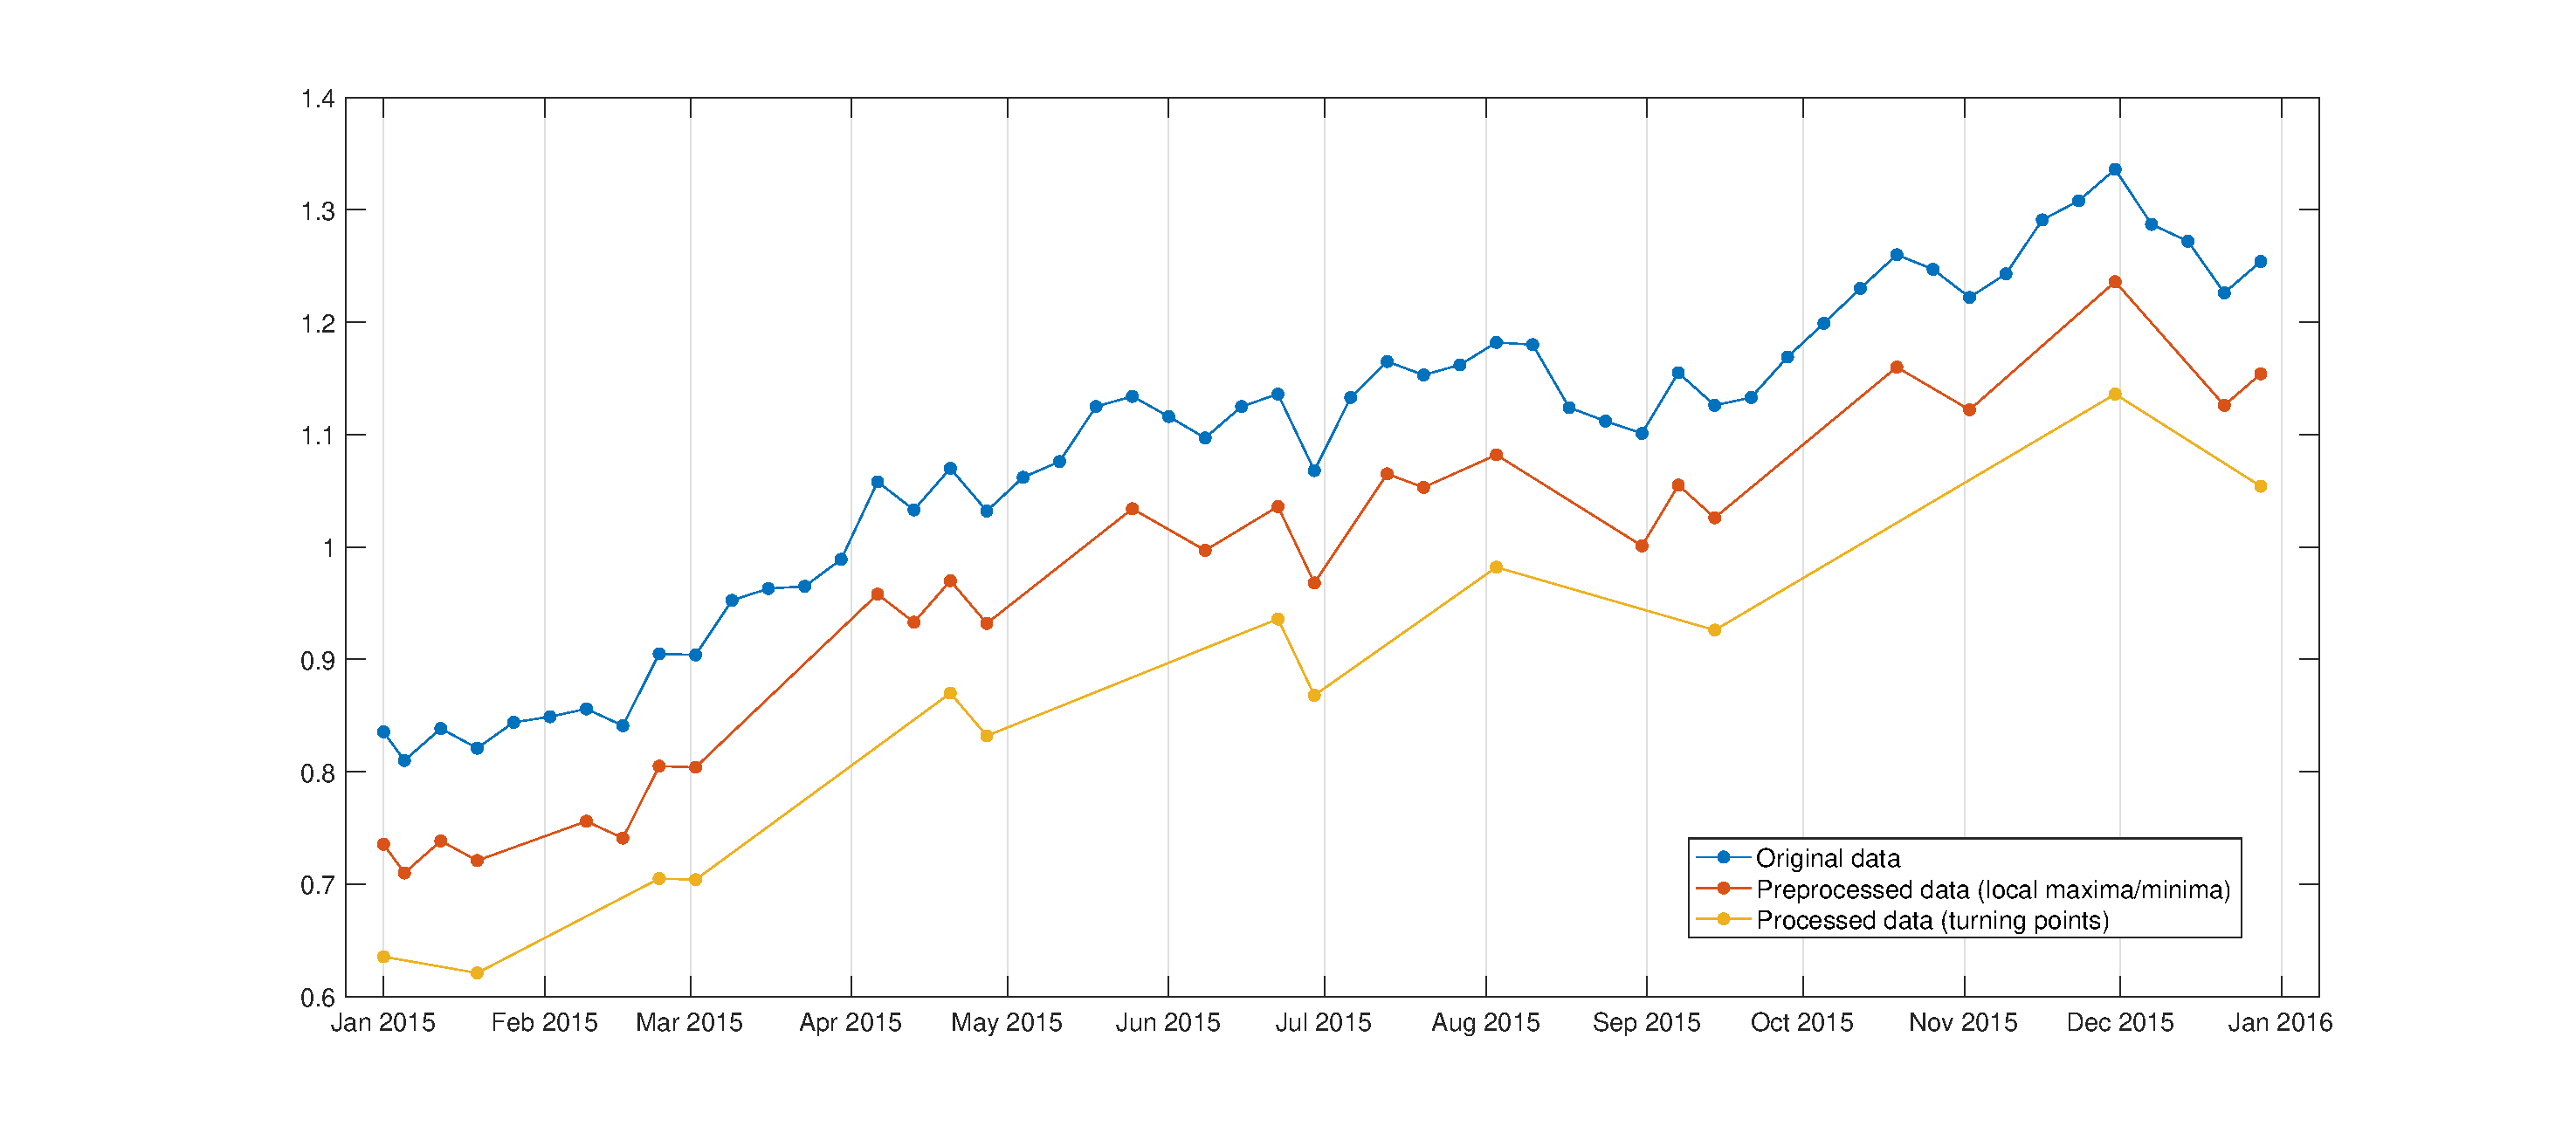
\includegraphics[width=1.8\textwidth]{img/a2a_W_15}}
	
	\caption{\texttt{A2A.MI} weekly 2015. Original data is in the correct position. The other two series are shifted down by 0.1 each.}\label{fig:a2a_w_2015}

\end{figure}


\subsection{Turning points in Python}\label{sec:tp_python}
\lipsum[1-3]



\subsection{Other implementations}\label{sec:other}
\lipsum[4-6]





%TODO Sistema.
\clearpage
\defbibnote{prenote}{DOI (Digital Object Identifier), when defined, serves as URL to retrieve the document. Documents may be accessible only on institutional log in (e.g., academic credentials).}
\nocite{*}
\printbibliography[title={Bibliography}, prenote=prenote] 


\end{document}







